 \documentclass[12pt, letterpaper]{article}
 \usepackage[utf8]{inputenc}
 \usepackage{geometry}
 \usepackage{graphicx}
 \usepackage{multirow}
 \usepackage{subfig}

 \geometry{letterpaper, margin=1.2in}
 \graphicspath{ {./images/}  }

 \title{Clinical drug response prediction using Lasso\\ \large{ECSE 556 - Machine Learning in Network Biology} \\ \large{Homework 1}}
 \author{Yazdan Zinati\\yazdan.zinati@mail.mcgill.ca\\ 260928077}
 \date{\today}

 \begin{document}
 \maketitle
 \newpage
 \section*{Introduction}
 Cancer is a preeminent cause of death worldwide \cite{bray2018global}. Until recently, cancer treatments were solely chosen based on the cancer type and administered to all patients with a specific type of cancer. However, recent methods consider patient's genomic data for choosing cancer treatment \cite{twomey2017drug}. Machine Learning models have been developed to predict drug responses of cancer cell lines (CCL) \cite{10.1093/bib/bbw065}. Nonetheless, one problem they face is the lack of sufficient samples. 
 In this study, we use transcriptomic data from the Genomics of Drug Sensitivity in Cancer (GDSC) dataset containing gene expression and drug response data of cancer cell lines to predict the clinical drug response (CDR) of cancer patients. This study will ultimately improve our understanding of features that affect CCLs and will enable us to ensure more reliable patient care by tailoring cancer monotherapy to individuals and ensure more effective drug responses.  
 
 \section*{Preprocessing and data exploration}

The GDSC gene expression dataset contains 13940 genes and 979 samples. As is the case with most transcriptomic datasets, we are facing the curse of dimensionality. The limited number of samples is one of the main bottlenecks in computational biology research. However, we will attempt to tackle this problem using Lasso in a later section. 

Since libraries that we will use later assume that features (genes) correspond to columns and samples (cell lines) correspond to rows in our data frame, which is not the case in transcriptomic datasets, we transpose our data frame. 

 Next, we perform Z-score normalization by scaling and centering independently on each gene as genes have different baseline expressions. the standard score of a sample $x$ is calculated using the equation bellow where $u$ and $s$ are the mean and standard deviation of the training samples. 
$$z = \frac{(x - u)}{s}$$


Feature scaling is necessary in our case as we intend to perform dimensionality reduction, clustering, and regularized regression. PCA assigns more weight to variables with larger variance. Applying Z-score normalization will improve its performance as features will no longer have a different variance. When it comes to clustering, some rely on the distance between observations. A feature on a different scale than others might overly influence distance measures. Finally, as Lasso puts a constraint on coefficients associated with variables, a variable with a large magnitude will dominate and make the estimator incapable of learning from the rest of the features.
Thus, this step is necessary to get the best performance in the tasks we are performing.  
\section*{Dimensionality reduction}
In this step, we visualize the high dimensional transcriptomic data using dimensionality reduction and map samples into a two-dimensional space. We use three different dimensionality reduction methods (PCA, t-SNE, and UMAP) and compare them. 
\\
Starting with PCA, we intend to select the principal components that are the most informative. To analyze the performance of PCA on our dataset, we examine the amount of variance explained by each principal component vector graphically through a scree plot. This scree plot is shown in Figure 1. Contrary to the ideal scree plot in which the first components explain most of the variability and the rest explain small fractions, our first component only explains 8\% of the explained variance, with the second PC explaining just about 4\%. Therefore, PCA would not perform well on our dataset if we for purposes other than visualization. However, as our goal is to visualize data in two-dimensional space, we choose the first two components. 

\begin{figure}[h]
    \centering
    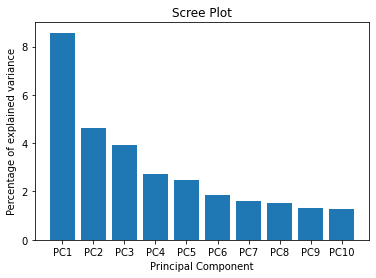
\includegraphics[scale=0.5]{scree_plot.png}
    \caption{PCA scree plot}
\end{figure}

Principal Component Analysis (PCA) is a linear dimensionality reduction technique. On the contrary, UMAP (Uniform Manifold Approximation and Projection) and t-SNE (t-distributed stochastic neighbor embedding) are non-linear dimensionality reduction techniques. As a result, PCA performs poorly on non-linear data due to being incapable of identifying complex non-linear relationships in the data. It can be influenced by the presence of outliers in the data. PCA does not involve hyperparameters which is an advantage over UMAP and t-SNE. From the three techniques, PCA is the least computationally expensive technique. UMAP is the second-best method in terms of time and space complexity. In our experiment, we found that a single run of each method took 0.6s, 6.3s, and 17s for PCA, t-SNE, and UMAP respectively. Even thought t-SNE outperformed UMAP in terms of runtime in our experiment, it is most likely due to the used parameters provided when calling the method, implementation details, or GPU parallelization. t-SNE is highly inefficient for large datasets as it computes pairwise conditional probabilities for each data point while trying to minimize the sum of the difference of the probabilities in higher and lower dimensions. Therefore, it scales quadratically and becomes impractical to use in large datasets. It is a common practice to use PCA to reduce features to a reasonable number before applying t-SNE to tackle this problem. UMAP does not need this preprocessing step like t-SNE when applied on large datasets. UMAP and PCA also have the advantage of being deterministic over t-SNE. The same output can be received on each run of the method. One of the main differences between the three dimensionality reduction methods is how they preserve local and global structures of the data. In summary, PCA is better at preserving the global structure, while t-SNE is better at preserving the local structure. UMAP is claimed to preserve the local structure and most of the global structure in the data. the goal of PCA is to find the directions that maximize the variance in a dataset. Therefore, it does not preserve local neighborhoods, unlike t-SNE. The lack of preservation of global structure in t-SNE means that the distance between formed clusters is not interpretable. Two similar clusters are not necessarily at closer distances than two dissimilar ones.
\\

Visually, we can see the formation of different clusters after performing dimensionality reduction on the dataset. This two-dimensional visualization is shown in Figure 2. We can clearly see the formation of three clusters in the UMAP visualization. It is slightly harder to distinguish the formed clusters in PCA and t-SNE as they are not as distanced as in the UMAP visualization. It should be noted that UMAP clusters are not only better separated than those formed by t-SNE and PCA but are also denser. Nonetheless, what we can see in all three visualizations is the presence of a large cluster and two smaller ones. In all three 2d visualizations, the larger cluster is close to one of the smaller clusters and separated by a distance from the third one. 
UMAP and t-SNE visualizations could have significantly changed based on the choice of parameters. In this study, we did not optimize the parameters for any of the dimensionality methods applied. 
\begin{figure}[h]
    \centering
    \subfloat[\centering PCA]{{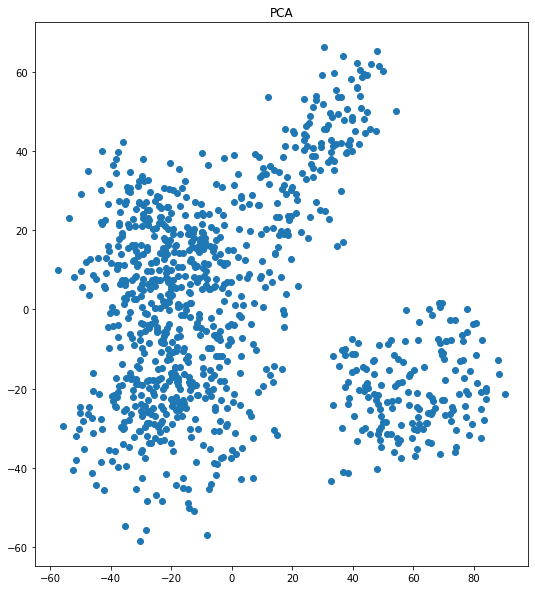
\includegraphics[width = 0.305\textwidth]{dimensionality_reduction_PCA.png} }}%
    \quad
    \subfloat[\centering t-SNE]{{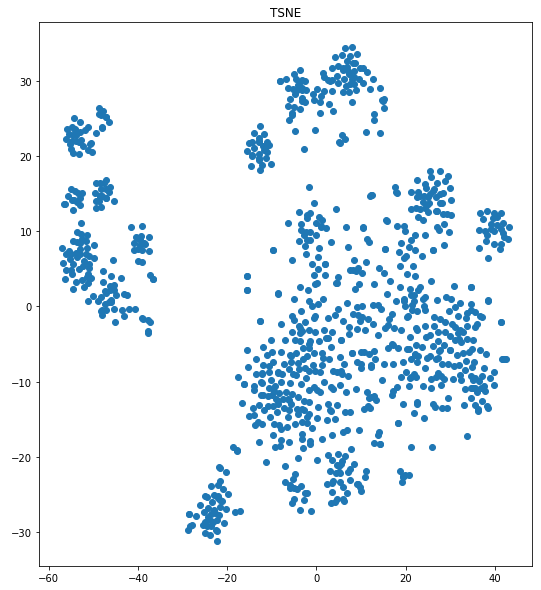
\includegraphics[width = 0.305\textwidth]{dimensionality_reduction_tSNE.png} }}
    \quad
    \subfloat[\centering UMAP]{{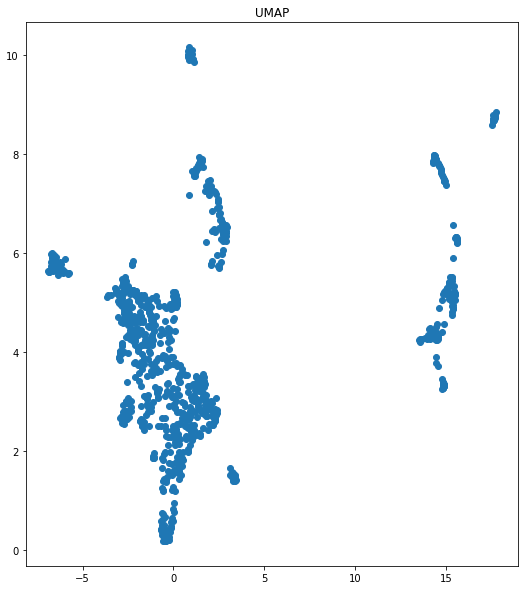
\includegraphics[width = 0.305\textwidth]{dimensionality_reduction_UMAP.png} }}%
    \caption{Two-dimensional visualization of the dataset using dimensionality reduction}
\end{figure}

\section*{Clustering}
\begin{figure}[h]
    \centering
    \subfloat[\centering Silhouette plot]{{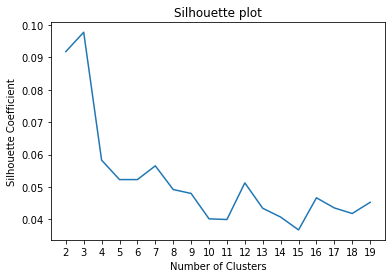
\includegraphics[width = 0.45\textwidth]{silhouette_plot_kmeans.png} }}%
    \quad
    \subfloat[\centering Knee plot]{{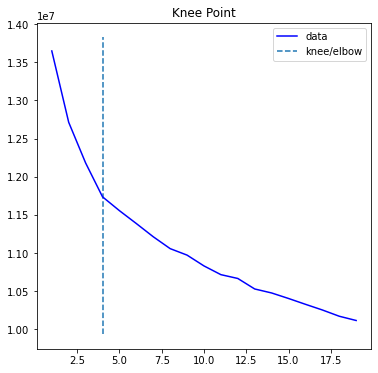
\includegraphics[width = 0.35\textwidth]{knee_plot_kmeans.png} }}
    \caption{K-means clustering exploration plots}
\end{figure}
\begin{figure}[h]
    \centering
    \subfloat[\centering PCA]{{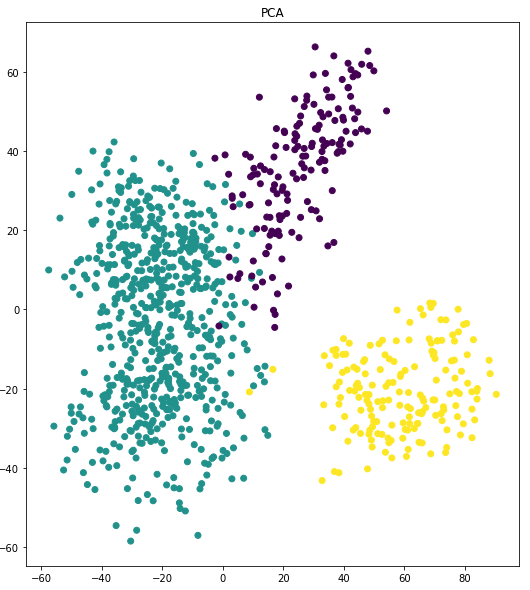
\includegraphics[width = 0.305\textwidth]{kmeans_PCA.png} }}%
    \quad
    \subfloat[\centering t-SNE]{{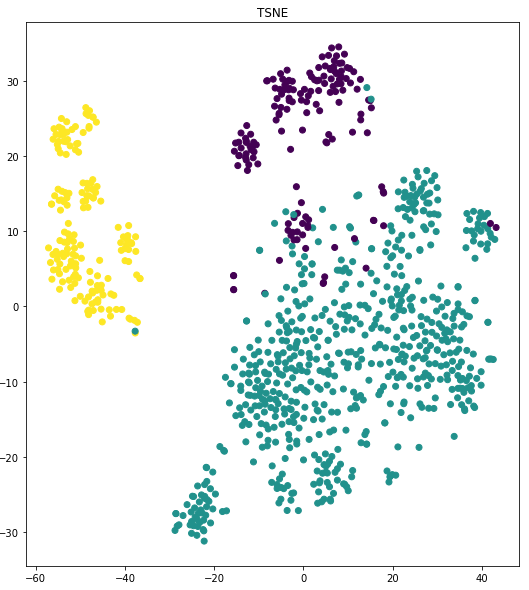
\includegraphics[width = 0.305\textwidth]{kmeans_tSNE.png} }}
    \quad
    \subfloat[\centering UMAP]{{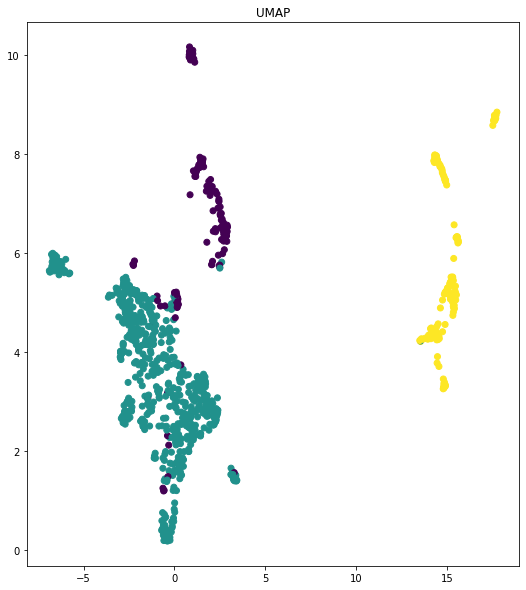
\includegraphics[width = 0.305\textwidth]{kmeans_UMAP.png} }}%
    \caption{Two-dimensional visualization of the dataset clustered using k-means}
\end{figure}
\begin{figure}[h]
    \centering
    \subfloat[\centering Silhouette plot]{{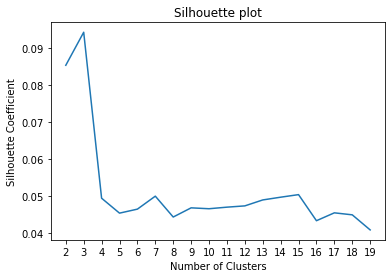
\includegraphics[width = 0.45\textwidth]{silhouette_plot_agglo.png} }}%
    \quad
    \subfloat[\centering Dendrogram]{{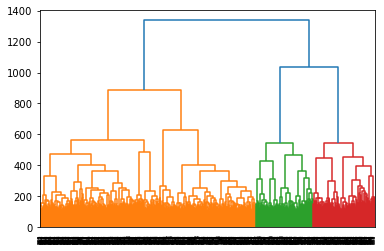
\includegraphics[width = 0.45\textwidth]{dendrogram_agglo.png} }}
    \caption{agglomerative clustering exploration plots}
\end{figure}
\begin{figure}[h]
    \centering
    \subfloat[\centering PCA]{{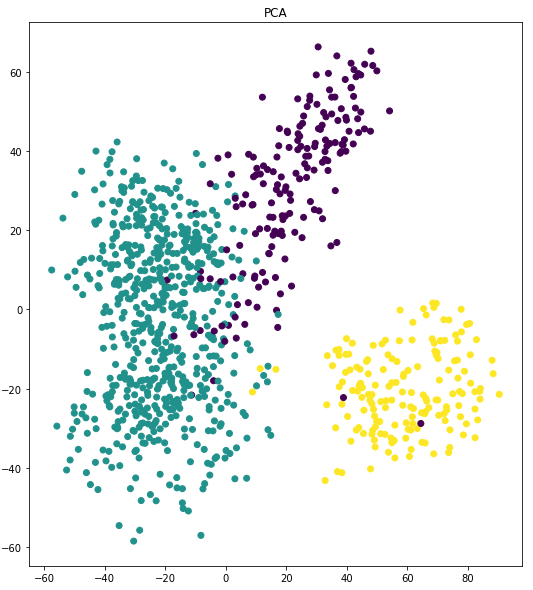
\includegraphics[width = 0.305\textwidth]{agglo_PCA.png} }}%
    \quad
    \subfloat[\centering t-SNE]{{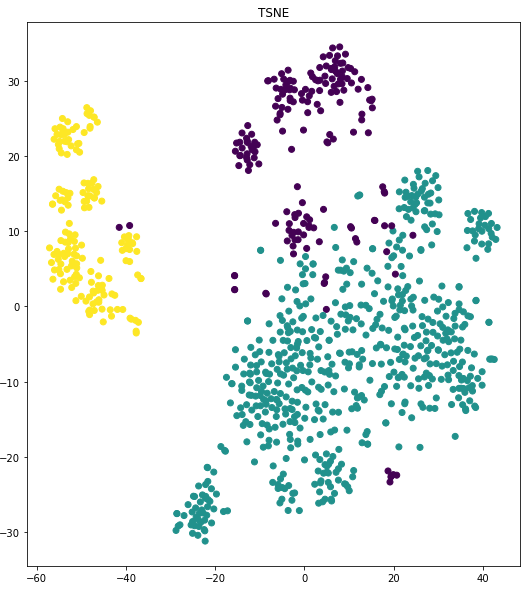
\includegraphics[width = 0.305\textwidth]{agglo_tSNE.png} }}
    \quad
    \subfloat[\centering UMAP]{{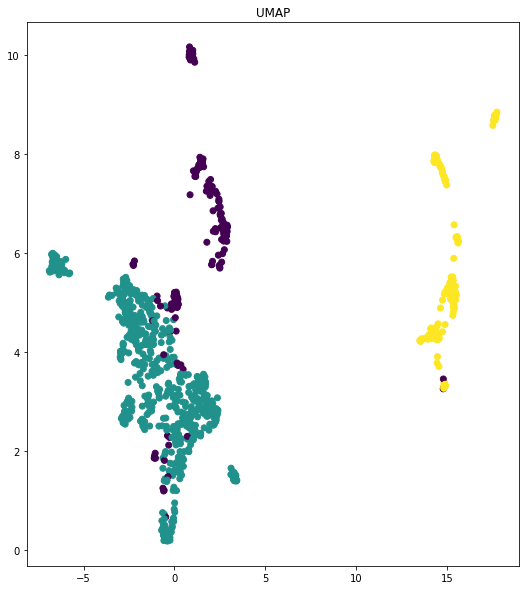
\includegraphics[width = 0.305\textwidth]{agglo_UMAP.png} }}%
    \caption{\centering Two-dimensional visualization of the dataset clustered using agglomerative clustering}
\end{figure}
\begin{figure}[h]
    \centering
    \subfloat[\centering kmeans/agglomerative clustering with default parameters]{{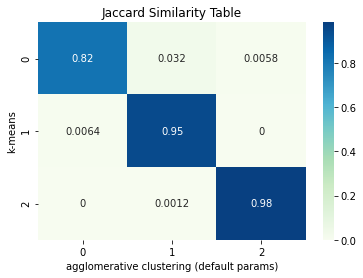
\includegraphics[width = 0.32\textwidth]{jaccard1.png} }}%
    \quad
    \subfloat[\centering kmeans/agglomerative clustering with average linkage and euclidean affinity]{{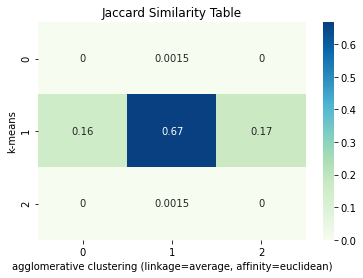
\includegraphics[width = 0.32\textwidth]{jaccard2.png} }}
    \quad
    \subfloat[\centering kmeans/agglomerative clustering with average linkage and cosine affinity]{{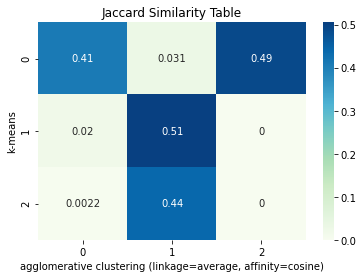
\includegraphics[width = 0.32\textwidth]{jaccard3.png} }}%
    \caption{\centering Jaccard similarity table - rows correspond to clusters formed using k-means and columns
    using agglomerative clustering}
\end{figure}
\begin{figure}[h]
    \centering
    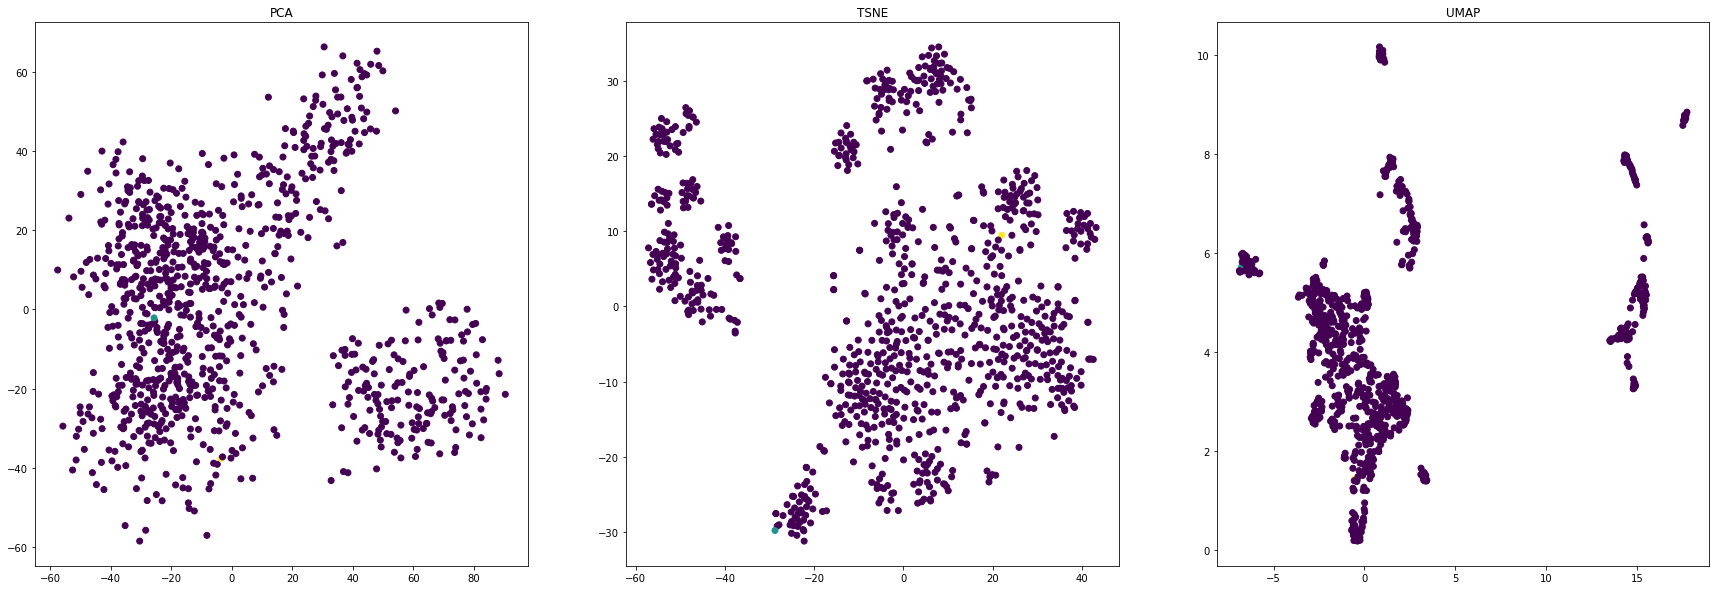
\includegraphics[width=\textwidth]{agglo2.png}
    \caption{\centering Two-dimensional visualization of the dataset clustered using agglomerative clustering with average linkage and euclidean affinity. \newline From left to right: PCA, t-SNE, UMAP.}
\end{figure}

\begin{figure}[h]
    \centering
    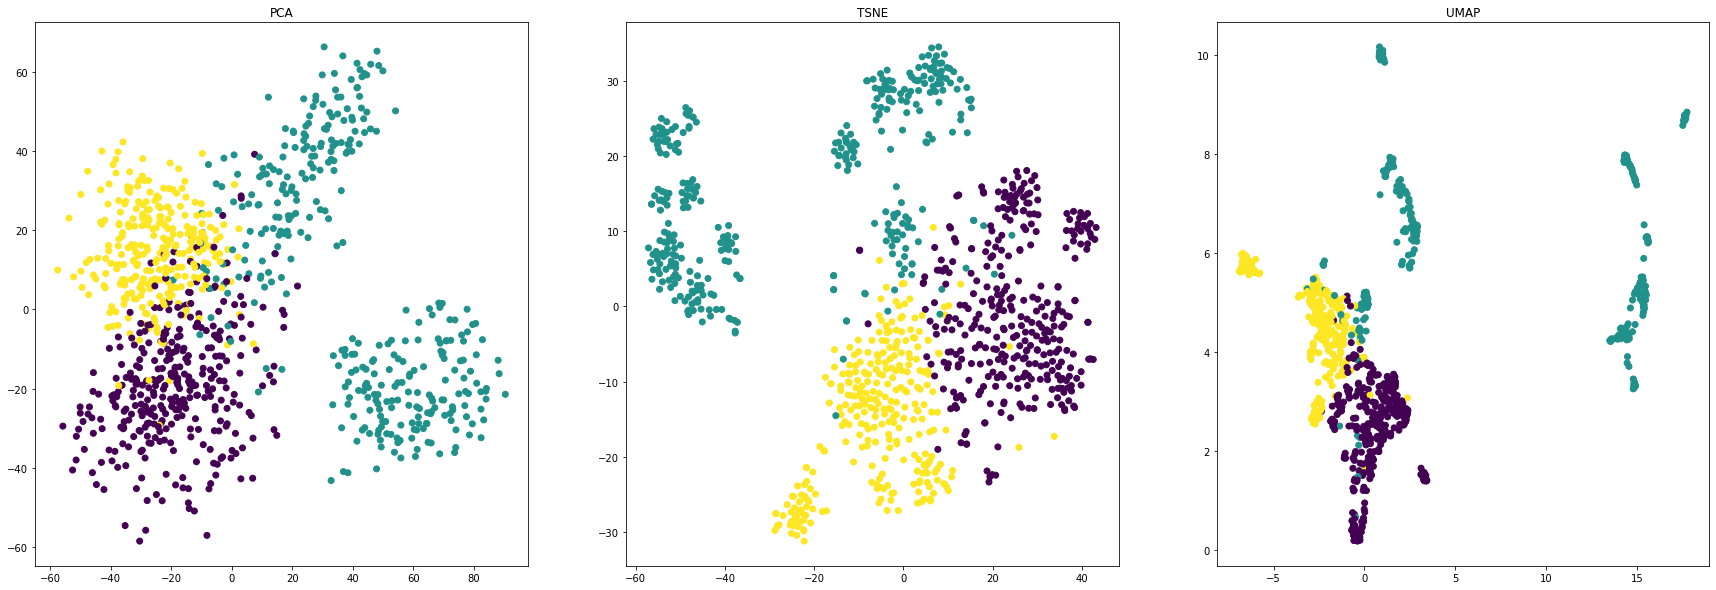
\includegraphics[width=\textwidth]{agglo3.png}
    \caption{\centering Two-dimensional visualization of the dataset clustered using agglomerative clustering with average linkage and cosine affinity. \newline From left to right: PCA, t-SNE, UMAP.}
\end{figure}
\clearpage

 \section*{Regression}

 In this step, we use linear and lasso regression to predict the clinical drug response based on gene expression profiles from the GDSC dataset. We are provided with a drug response file. This CSV file contains the response of cell lines to 23 different drugs. The rows contain drugs, and the columns represent cell lines. The drug we are interested in predicting the response of is Doxorubicin. Doxorubicin is a chemotherapy medication used in the treatment of different kinds of cancer \cite{drugs.com}. \\
 
 Before performing regression, we match the gene expression file to the drug responses. For this, we transpose the drug responses so each row corresponds to a cell line. Moreover, we remove any sample for which no response to Doxorubicin is recorded. This alone removes 107 cells lines and works against us due to the curse of dimensionality. Performing a regression using linear regression gives us an $r^{2}$ regression score of 1 on the training data, but an $r^{2}$ score close to zero on the test set. 
 This clearly shows that linear regression overfits the data. To combat this issue, we perform a regularized regression using Lasso. 
 We will penalize the features in the model to only keep the most important ones. This penalization is controlled using the $\alpha$ hyperparameter. We perform Lasso regression using values of $\alpha$ from 0.1 to 1 in increments of 0.2 and plot the number of selected features. This plot can be seen in Figure 10. 
 We can see that an $\alpha$ of 0.1 limits the features to 195m and the number of features decreases as $\alpha$ increases. The number of features is limited to only one with $\alpha$ larger or equal to 0.7. 
 \begin{figure}[h]
    \centering
    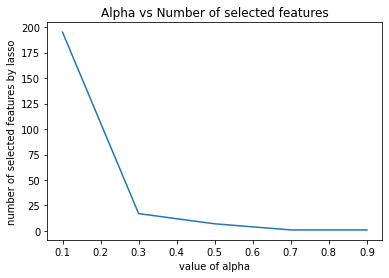
\includegraphics[width=0.5\textwidth]{alpha_vs_nfeatures.png}
    \caption{\centering Number of selected features by LASSO vs. the value of the $\alpha$ hyperparameter}
\end{figure}

Next, we perform nested cross-validation to tune the $\alpha$ hyperparameter and to estimate the model's generalization error. When performing cross-validation in a non-nested manner on the data for tunning and evaluating the model, data leakage might occur depending on the dataset, biasing the model. As a result, the model evaluation will be optimistic and biased. In nested cross-validation, we have an outer loop we use for assessing the model's performance and an inner loop for parameter selection. We perform 4-fold cross-validation on the outer loop and 3-fold cross-validation for the inner loop. This means that for each iteration of the outer loop, the outer training set is further split into 3 folds. We perform grid search with a mean squared error as score in the inner loop over $\alpha$ values from 0.02 to 1 with intervals of 0.01. We found that the best value of $\alpha$ was in the range of 0.2 to 0.3. From MSE scores reported in the outer loop, an $\alpha$ of 0.21 reported an MSE of 2.33. Using this an $\alpha$ of 0.21 resulted in a spearman correlation of 0.38. Note that we performed the nested cross-validation using MSE in the inner loop as the score and the score reported for spearman correlation does not come from the nested cross-validation. However, it is possible to repeat the same procedure for nested cross-validation replacing using spearman correlation as score. This wasn't done due to computational limitations. 

 \section*{Conclusion}
 \bibliographystyle{unsrt}
 \bibliography{refs}

 \end{document} 